
\documentclass{article}

\usepackage{mymathstyle} % math macros

\usepackage[dvipsnames]{xcolor}         % colors
\usepackage[utf8]{inputenc} % allow utf-8 input
\usepackage[T1]{fontenc}    % use 8-bit T1 fonts
\usepackage{hyperref}       % hyperlinks
\usepackage{url}            % simple URL typesetting
\usepackage{booktabs}       % professional-quality tables
\usepackage{amsfonts}       % blackboard math symbols
\usepackage{nicefrac}       % compact symbols for 1/2, etc.
\usepackage{microtype}      % microtypography
\usepackage[capitalize,noabbrev]{cleveref}
\usepackage{caption}
\usepackage{subcaption}
\usepackage{float}
% \usepackage{subfigure}
\usepackage{booktabs}
\usepackage{multirow}
\usepackage{multicol}
\usepackage{graphicx}
\usepackage{enumitem}

% Recommended, but optional, packages for figures and better typesetting:
% \usepackage{microtype}
% \usepackage{graphicx}
% \usepackage{subfigure}
% \usepackage{booktabs} % for professional tables

% hyperref makes hyperlinks in the resulting PDF.
% If your build breaks (sometimes temporarily if a hyperlink spans a page)
% please comment out the following usepackage line and replace
% \usepackage{icml2025} with \usepackage[nohyperref]{icml2025} above.
% \usepackage{hyperref}


% Attempt to make hyperref and algorithmic work together better:
% \newcommand{\theHalgorithm}{\arabic{algorithm}}

% Use the following line for the initial blind version submitted for review:
\usepackage[accepted]{icml2025}

% If accepted, instead use the following line for the camera-ready submission:
% \usepackage[accepted]{icml2025}

% For theorems and such
% \usepackage{amsmath}
% \usepackage{amssymb}
% \usepackage{mathtools}
% \usepackage{amsthm}

\usepackage{paper_commands}

\usepackage{algorithm2e}
\RestyleAlgo{ruled}

\crefname{algocf}{alg.}{algs.}
\Crefname{algocf}{Algorithm}{Algorithms}


% region set up fixme and in-text annotations
% \usepackage{pdfcomment}
% % put draft in options if, otherwise remove
% % \usepackage[draft, noinline, margin, mode=multiuser, author=]{fixme}
% \usepackage[noinline, margin, mode=multiuser, author=]{fixme}
% \usepackage[us]{datetime}
% \fxloadlayouts{pdfcnote}
% \fxuseenvlayout{colorsig} % plain, signature, color, colorsig
% \fxusetargetlayout{changebar} % plain, changebar, color, colorcb
% \FXRegisterAuthor{aa}{anaa}{\color{Violet}Awni}
% \FXRegisterAuthor{jl}{anjl}{\color{Magenta}John}
% \fxusetheme{colorsig}
% \fxsetface{margin}{\scriptsize}
% endregion

% region hyperref and link color options
% \newcommand\myshade{100}
% \colorlet{mylinkcolor}{RubineRed}
% \colorlet{mycitecolor}{RoyalBlue}
% \colorlet{myurlcolor}{RoyalBlue}

\hypersetup{
  linkcolor  = RubineRed, %mylinkcolor!\myshade!black,
  citecolor  = RoyalBlue, %!\myshade!black,
  urlcolor   = RoyalBlue, %!\myshade!black,
  colorlinks = true,
}
% endregion

% region biblatex bibliography setup
\usepackage[backend=bibtex, style=numeric-comp, url=false, isbn=false, doi=false, sorting=none, natbib=true, backref=true]{biblatex}
% \usepackage[backend=bibtex, style=authoryear-comp, date=year, maxbibnames=10, maxcitenames=2, url=false, uniquelist=false, isbn=false, doi=false, sortcites=false, dashed=false, natbib=true, backref=true]{biblatex}
\DefineBibliographyStrings{english}{%
  backrefpage = {cited on page},% originally "cited on page"
  backrefpages = {cited on pages},% originally "cited on pages"
}
\AtEveryBibitem{%
  \clearfield{volume}%
  \clearfield{number}
  \clearfield{pages}}
\DeclareFieldFormat{title}{\mkbibquote{#1}}
\addbibresource{references.bib}
% endregion

\newcommand{\edit}[1]{\textcolor{Bittersweet}{#1}} % to highlight passages that can/should revised
\newcommand{\trim}[1]{\textcolor{OrangeRed}{#1}} % to highlight passages that can perhaps be trimmed or removed
\newcommand{\todo}[1]{\textcolor{PineGreen}{#1}} % for in-line notes about things i need to do

% \def\baselinestretch{0.95} % 0.92 also looks fine

\icmltitlerunning{Relational \& Sensory Processing in Transformers}

\begin{document}

\twocolumn[
\icmltitle{Disentangling and Integrating Relational and Sensory \\Information in Transformer Architectures}

\begin{icmlauthorlist}
\icmlauthor{Awni Altabaa}{yale}
% \icmlauthor{John Lafferty}{yale,wti}
\icmlauthor{John Lafferty}{yalewti}
\end{icmlauthorlist}

\icmlaffiliation{yale}{Department of Statistics and Data Science, Yale University}
% \icmlaffiliation{wti}{Wu Tsai Institute}
\icmlaffiliation{yalewti}{Department of Statistics and Data Science, Wu Tsai Institute, Yale University}

\icmlcorrespondingauthor{Awni Altabaa}{awni.altabaa@yale.edu}
\icmlcorrespondingauthor{John Lafferty}{john.lafferty@yale.edu}

% You may provide any keywords that you
% find helpful for describing your paper; these are used to populate
% the "keywords" metadata in the PDF but will not be shown in the document
\icmlkeywords{relational, reasoning, attention, transformers, inductive biases, sensory, relational, architecture, attention}

\vskip 0.3in
]

% this must go after the closing bracket ] following \twocolumn[ ...

% This command actually creates the footnote in the first column
% listing the affiliations and the copyright notice.
% The command takes one argument, which is text to display at the start of the footnote.
% The \icmlEqualContribution command is standard text for equal contribution.
% Remove it (just {}) if you do not need this facility.

\printAffiliationsAndNotice{}  % leave blank if no need to mention equal contribution
% \printAffiliationsAndNotice{\icmlEqualContribution} % otherwise use the standard text.

\input{abstract.tex}

% \tableofcontents

% \newpage

\section{Introduction}\label{sec:intro}

A central goal of machine learning research is to develop a universal architecture capable of learning and reasoning across a wide range of tasks and data modalities. Theoretical frameworks for understanding human and animal intelligence seek to explain intelligent behavior through a small set of fundamental principles~\citep{marcus2003algebraic}. However, in machine intelligence, there is a tension between the objective of developing a \textit{general} architecture and the need to incorporate \textit{inductive biases} that are beneficial for specific tasks~\citep{wolpert1995no,baxter2000model}. When faced with finite training data and numerous solutions to empirical risk minimization, inductive biases steer the learning algorithm towards solutions with desirable properties, enhancing data efficiency and generalization.
A core scientific challenge of machine learning is to identify a complete and broadly applicable set of inductive biases that promote robust, flexible, and data-efficient learning across a diverse set of problems.
% There is, however, a tension between the goal of creating a general architecture and the need to incorporate inductive biases that are beneficial for specific tasks~\citep{wolpert1995no,baxter2000model}.
% In machine intelligence, the scientific challenge is to identify a complete set of fundamental inductive biases with broad applicability to real-world problems that enable robust, flexible, and data-efficient learning.

Relational reasoning is a central component of generally intelligent systems and is believed to underlie human abilities for abstraction and systematic generalization~\citep{gentner1983structure,snow1984topography,kemp2008discovery,holyoak2012analogy}. The power of relational reasoning lies in its capacity to generate inferences and generalizations in systematic and novel ways, even across instances which are superficially very different but have similarities on an abstract structural level. This grants humans a capacity for out-of-distribution generalization, data efficiency, and continual learning, which modern machine learning is yet to match~\citep{lake2017building,smith2019promise,nogueira2021investigatinglimitationstransformerssimple}. Replicating this ability in machine intelligence can ultimately lead to universal inductive generalization from a finite set of observations to an infinite set of novel instances~\citep{goyal2022inductive}.

The ability of artificial intelligence systems to perform relational reasoning has long been an area of active study across various approaches to AI. In symbolic modeling frameworks, the relationships between symbols are explicitly defined in the language of logic and mathematics~\citep{newell1980physical,harnad1990symbol,fodor1988connectionism}. However, such approaches often require hand-crafted representations and suffer from the symbol grounding problem, limiting their ability to generalize to variations in the task or input outside a certain domain. By contrast, deep learning approaches build data-dependent representations that are, in principle, capable of generalizing across diverse conditions. However, recent work exploring the ability of deep learning models to learn relational tasks finds that seemingly simple relational inferences can be remarkably difficult for powerful neural network architectures~\citep{lake2018generalization,barrett2018measuring,hill2018learning,webbEmergentSymbolsBinding2021,santoroSimpleNeuralNetwork2017,shanahanExplicitlyRelationalNeurala,kergNeuralArchitectureInductive2022,altabaa2024abstractors,altabaaLearningHierarchicalRelational2024}. An emerging hypothesis, which we explore further here, explains this through the lens of inductive biases, arguing that neural networks struggle with relational reasoning because they overemphasize individual object representations---\textit{sensory} information---while lacking \textit{explicit} mechanisms for encoding and processing \textit{relational information}~\citep{webbRelationalBottleneckInductive2024}.

In this work, we explore this idea in the context of the Transformer architecture~\citep{vaswani2017attention}, which offers a promising starting point for building a versatile, general-purpose neural architecture. Although Transformers, like other neural architectures, struggle to learn abstract relational representations~\citep{santoroSimpleNeuralNetwork2017,shanahanExplicitlyRelationalNeurala,kergNeuralArchitectureInductive2022,altabaa2024abstractors,altabaaLearningHierarchicalRelational2024}, there is encouraging evidence that Transformer-based foundation models acquire some relational reasoning ability~\citep{wei2022chain,kojima2022large,valmeekam2022large,huang2023reasoninglargelanguagemodels,webb2023emergent,huang2024largelanguagemodelsselfcorrect,mirzadeh2024gsmsymbolicunderstandinglimitationsmathematical} through large-scale training on large amounts of data~\citep{brown2020languagemodelsfewshotlearners,kaplan2020scalinglawsneurallanguage,hoffmann2022trainingcomputeoptimallargelanguage,grattafiori2024llama3herdmodels}. This presents an opportunity to explore Transformer-based architectures with built-in neural mechanisms and inductive biases for explicit and enhanced relational reasoning capabilities, seeking to imbue the Transformer architecture with a greater capacity for efficient induction of abstractions.

To introduce our proposal, we highlight a distinction between two types of information which are encoded in the internal representation of Transformer models: \textit{sensory information}, which represents features of individual objects, and \textit{relational information}, representing comparisons and relationships between objects. In the standard attention mechanism of Transformers, relational information is \textit{entangled} with sensory information, limiting the model's ability to learn to explicitly represent and reason about the relationships between objects. In particular, in standard attention, relational information \textit{directs} the flow of information (i.e., attention scores encoding a selection criterion), while the \textit{values} routed are representations of the sensory attributes of individual objects. In this work, we explore a new type of attention mechanism we call \textit{relational attention}, in which the values being routed are themselves representations of relationships between the source and the target, computed explicitly as a series of comparisons under learned feature maps. This equips the model with a mechanism for explicitly routing and processing relational information, decoupling it from sensory features.

We integrate relational attention with the standard attention mechanism of Transformers, yielding a variant of multi-head attention that processes both sensory and relational information in parallel. The resulting \textit{Dual Attention Transformer (DAT)} architecture disentangles the two types of information during the information retrieval stage and integrates them during the local processing stage of each layer. We empirically evaluate this architecture on a diverse set of tasks, ranging from synthetic benchmarks on relational reasoning to complex real-world tasks such as language modeling and visual processing. Our results demonstrate that integrating explicit relational mechanisms into the Transformer architecture leads to significant performance gains in terms of data efficiency and parameter efficiency.

\begin{figure*}
  \centering
  \begin{subfigure}[t]{0.415384615\textwidth} % 0.9 * 3 / 6.5
    \centering
    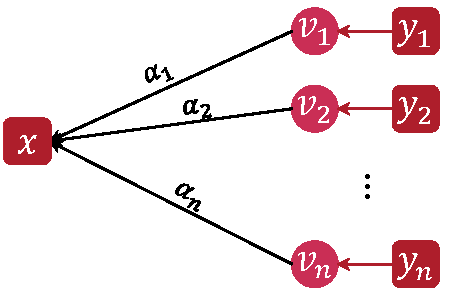
\includegraphics[width=0.8\textwidth]{figs/sensory_retrieval.pdf} % size: 3 x 2 in
    \caption{$\Attn(x, \ys)$}%: Retrieval of sensory information by standard attention.}
  \end{subfigure}
  \qquad
  \begin{subfigure}[t]{0.484615385\textwidth} % 0.9 * 3.5 / 6.5
    \centering
    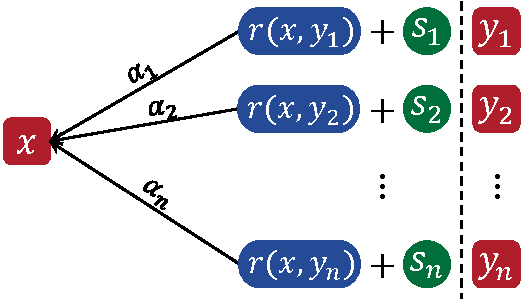
\includegraphics[width=0.8\textwidth]{figs/relational_retrieval.pdf} % size 3.5 x 2 in
    \caption{$\RelAttn(x, \ys)$}%: Retrieval of relational information by relational attention.}
  \end{subfigure}
  % 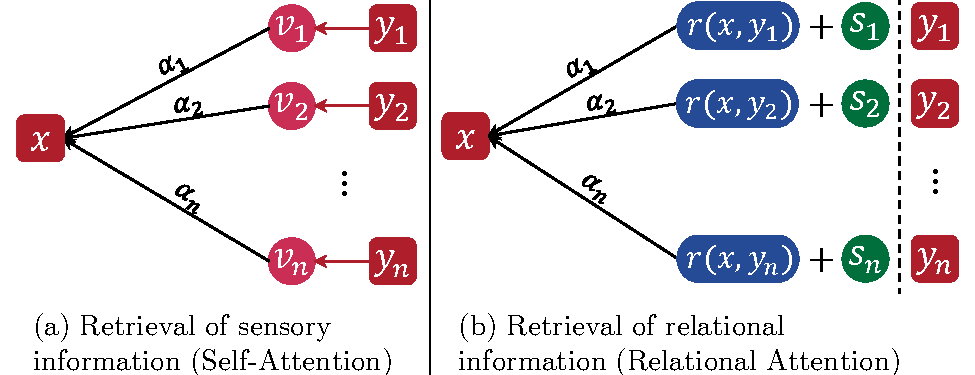
\includegraphics[width=0.8\textwidth]{figs/attn_fig_combined_noqeuerykey.pdf}
  \caption{Standard self-attention retrieves sensory information $v_i$ about the attributes of individual objects while relational attention retrieves relational information $r(x, y_i)$ about the relationship between the objects in the context and the target.
  Each relation is tagged with a symbol $s_i$ which acts as an abstract variable identifying the source.
  In both cases, information is aggregated according to the attention scores $\alpha_i$, which are computed by a softmax over inner products of queries and keys.
  }\label{fig:selfattn_relattn}
  % \vskip-12pt
\end{figure*}


% \section{Related Work}

\aawarning{TODO---use~\citep{santoroSimpleNeuralNetwork2017,santoroRelationalRecurrentNeural2018,webbEmergentSymbolsBinding2021} for relevant OG references.}

\begin{itemize}
    \item The ability for neural networks to learn to perform relational reasoning in a data-efficient manner while achieving generalization through the right types of abstractions.
    \item This is an ability humans possess, but which neural models struggle with (in terms of efficiency).
    \item One theory, which can be described in the language of ``inductive biases'', that has emerged for this pertains to the distinction between so-called ``sensory'' and ``relational'' information. Modern neural architectures generally lack explicit computational mechanisms for computing feature representations that explicitly encode relational information (that is, comparisons). Although neural models can learn to fit their data on relational tasks given enough data, this lack of relational inductive bias results in limited generalization and requires large amounts of data.
    \item More recently, there has been a significant amount of work evaluating the relational reasoning abilities of large language models based on the Transformer architecture. This work finds that some level of relational reasoning ability is attained in large models after injesting large amounts of data. Moreover, there is evidence that the internal representations come to encode interpretable relational representations.
    \item In response, a recent line of work studied the problem of designing neural architectures for enhanced relational reasoning, seeking to embed relational inductive biases which drive the model to discover solutions which generalize better with less data.
    \item An early example is~\citep{santoroSimpleNeuralNetwork2017} which ... .
    \item More examples...
    \item The most related work to ours is ~\citep{altabaa2024abstractors} which proposes an attention mechanism where the values are replaced by ..., 
    \item Previous work has been more restricted in domain, and mainly applied to synthetic relational benchmarks. The goal of the present work is ...
    \item Relationship to symbolic approaches to AI, which are inherently relational.
\end{itemize}

\input{disentangling_attention.tex}

\input{architectures.tex}

\input{experiments.tex}

\input{discussion.tex}

\input{reproducibility.tex}

\input{acknowledgment.tex}

\section*{Impact Statement}
This paper presents work whose goal is to advance the field of Machine Learning. There are many potential societal consequences of our work, none which we feel must be specifically highlighted here.

\printbibliography


% \listoffixmes


%%%%%%%%%%%%%%%%%%%%%%%%%%%%%%%%%%%%%%%%%%%%%%%%%%%%%%%%%%%%
\clearpage
\newpage
\appendix
\onecolumn

\input{approx.tex}

\clearpage
\input{implementation.tex}

\clearpage
\input{experiment_details.tex}

\clearpage
\input{comparison_og_abstractor.tex}

% \clearpage
% \newpage
% \input{nips_checklist.tex}

\end{document}